
\documentclass[oneside,12pt]{Latex/Classes/Thesis_Class_File}

\usepackage{enumitem}
\usepackage{pdfpages}
\usepackage{amssymb}
\usepackage{graphicx}
\usepackage{longtable}
\usepackage{lipsum}
\usepackage{tabularx}
\usepackage{multirow}
\usepackage{subfigure}
\usepackage{cite}
\usepackage{booktabs}
\usepackage{flushend}
\usepackage{multirow}
\usepackage{amsmath}
\usepackage{mathtools}
\usepackage{setspace}
\usepackage{color,soul}
\usepackage{glossaries}
\usepackage{comment}
\usepackage{url}
\usepackage{breakurl}
\usepackage{lscape}
\usepackage{array}
\usepackage{slashbox}
\usepackage{sectsty}
\usepackage{hyperref}
\usepackage{cite}
\usepackage{epstopdf}
\usepackage{float}
\usepackage[compact]{titlesec}  
\chapterfont{\centering}
\usepackage[inner=2.54cm,outer=2.54cm,bottom=2.54cm,top=2.54cm]{geometry}
\usepackage{layout}
\usepackage{bbding}
\usepackage{ulem}
\usepackage{xcolor}

\crest{\includegraphics[width=\textwidth,height=0.2\textheight]}

\title{\textbf{\LARGE CCE535 Graduation Project (1)\\ \vspace{10mm} `` Radar System Design''}}

\ifpdf
  \collegeordept{{Program of }\href{https://feng.bu.edu.eg/index.php/programs/special-new-programs/communication-computer-program}{Communication and Computer Engineering Program}}
  \university{\href{https://feng.bu.edu.eg/}{Faculty of Engineering at Shoubra}, \href{https://bu.edu.eg/}{Benha University}}
\fi
\degree{In Partial Fulfillment of the Requirements for the Degree of \\\vspace{3mm}\Large{Bachelor of Science}\\\vspace{10mm}\normalsize{in}\\\vspace{3mm}\Large{Communication and Computer Engineering Program\\}}
\degreedate{winter 2023}

\linespread{1.5}

\begin{document}

% Sets line spacing
\renewcommand\baselinestretch{1.2}
\baselineskip=18pt plus1pt

%: ---------- generate cover page -------------

\maketitle 
% command to print the title page with above variables

%: --------- cover page back side -------------

\newpage\null\thispagestyle{empty}\newpage
\thispagestyle{empty}

\begin{center}
{\setlength{\baselineskip}{1.5\baselineskip}
\textbf{\LARGE Advanced Computer Networks }
\par}
\end{center}
\vspace*{5mm}
\begin{center}
	\textbf{\underline{Student's Team Members}}
\end{center}
\begin{tabular}{p{10cm} p{5cm}}  
% p means normal cells
% b means alignment at the bottom
% m means alignment in the vertical center
\textbf{Name}  & \textbf{Student's ID} \\
Mohamed Rafaat Awad Awad & 231903353 \\
Shady Mohamed & 23190

\end{tabular}
\vspace*{3mm}
\begin{center}
	\textbf{\underline{Supervision Committee}}
\end{center}
\vspace*{3mm}
\begin{tabular}{p{12cm}  p{5cm}}
\textbf{Name, Title} & \textbf{Approved, Date} \\
Prof. Mohamed Salah Ahmed Selmy  & \ldots\ldots\ldots\ldots\ldots\ldots\ldots\ldots \\
Dr.  Mohamed Salah Ahmed Selmy  &\ldots\ldots\ldots\ldots\ldots\ldots\ldots\ldots \\
\end{tabular}
\vspace*{3mm}
\begin{center}
	\textbf{\underline{Examination Committee}}
\end{center}
\vspace*{3mm}
\begin{tabular}{p{7cm}  p{5cm} p{5cm}}
	\textbf{Name, Title} & \textbf{Affiliation} & \textbf{Approved, Date} \\
	\ldots\ldots\ldots\ldots\ldots\ldots & \ldots\ldots\ldots\ldots\ldots\ldots & \ldots\ldots\ldots\ldots\ldots\ldots\ldots\ldots \\
	\ldots\ldots\ldots\ldots\ldots\ldots & \ldots\ldots\ldots\ldots\ldots\ldots &\ldots\ldots\ldots\ldots\ldots\ldots\ldots\ldots \\
	\ldots\ldots\ldots\ldots\ldots\ldots & \ldots\ldots\ldots\ldots\ldots\ldots &\ldots\ldots\ldots\ldots\ldots\ldots\ldots\ldots \\
	\ldots\ldots\ldots\ldots\ldots\ldots & \ldots\ldots\ldots\ldots\ldots\ldots &\ldots\ldots\ldots\ldots\ldots\ldots\ldots\ldots \\
\end{tabular}
% =============================================
\newpage\null\thispagestyle{empty}\newpage

\addcontentsline{toc}{chapter}{SUMMARY}



\begin{abstract}       
 
This project covers aspects of ...................... 

\end{abstract}



% ----------------------------------------------
\newpage\null\thispagestyle{empty}\newpage
\addcontentsline{toc}{chapter}{ACKNOWLEDGMENT}

\begin{acknowledgment}      

\begin{center}
\textit{First of all, countless thanks to ALLAH the almighty} 
\end{center}
\vspace{5mm}

I would like to thank ......\\

\hfill Project Team Members

\end{acknowledgment}
%\end{acknowledgmentslong}

% ------------------------------------------------------------------------



\newpage\null\thispagestyle{empty}\newpage
\phantomsection
\addcontentsline{toc}{chapter}{TABLE OF CONTENTS}

%: ---------- contents ------------

\renewcommand{\contentsname}{TABLE OF CONTENTS}
{\tableofcontents} % print the table of contents

%: -------list of figures/tables ------------

\renewcommand{\listtablename}{LIST OF TABLES}
\renewcommand{\listfigurename}{LIST OF FIGURES}

\listoftables   % print list of tables
\listoffigures	% print list of figures
\cleardoublepage
\phantomsection
\addcontentsline{toc}{chapter}{NOMENCLATURE}
\begin{Symbols}
	
\begin{longtable}{m{3cm}   m{12cm}}
\($$b_f$$\) & The motor friction coefficient.\\
\($$e_a$, $e_b$ and $e_c$$\) & The trapezoidal induced emfs.\\
\($$\frac{d}{dt}$$\) & The derivative operator.\\
\end{longtable}

\end{Symbols}









\phantomsection
\addcontentsline{toc}{chapter}{ABBREVIATIONS} 

\begin{Abbreviations}
	
\begin{longtable}{m{3cm}   m{12cm}}
\(AMB\) & Active Magnetic Bearing.\\
\(BLDC\) & Brushless Direct Current.\\
\(CATIA\) & Computer Aided Three-dimensional Interactive Application\\
\end{longtable}

\end{Abbreviations}








\cleardoublepage
%: -----------MAIN DOCUMENT SECTION---------------

% define space before sections
\titlespacing{\section}{0pt}{10pt}{5pt}
\titlespacing{\subsection}{0pt}{10pt}{5pt}

\begin{spacing}{1.5}
	 % Use 1.5-space between lines.
	 
% the main text starts here with the introduction, 1st chapter,...

\mainmatter

%: -------------- subdocuments -----------------

% Parts of the thesis are included below. Rename the files as required.
% But take care that the paths match. You can also change the order of appearance by moving the include commands.


\chapter{INTRODUCTION}
\label{chapter:Intro}

%: ----------------------- paths to graphics ------------------------
\ifpdf
    \graphicspath{{1_Introduction/figures/PNG/}{1_Introduction/figures/PDF/}{1_Introduction/figures/}}
\else
    \graphicspath{{1_Introduction/figures/EPS/}{1_Introduction/figures/}}
\fi

% 
%: ----------------------- introduction content -----------------------


This project encompasses aspects of ...............Radar System design can control the rotor position with an accuracy of a micrometer \cite{Cleanroom}. 
\section{Project idea}
\noindent We are considering providing a complete radar system that
will help to reduce the number of accidents on the
highways by implementing a system that is used for car
speed detecting and fast recognizing the detail of the plate
of the car. This system is considered to be better than the
existing road radars and provide new features that will lead
to high accuracy, fast detecting, plate recognition and
plate's details extraction at every radar unit then send the
details to the responsible authority to take the necessary
action with the car driver. This System will meet our
specifications in a simple way with a simple radar circuit
that provide the signal for detecting the cars in an
electromagnetic wave, then make a simple hardware circuit
that provide the speed of the detected car by calibration to
give an order to the camera to picture the over speed cars.
After that the license plate of the car will be extracted from
the car picture and then extract the ARABIC letters and
numbers from the plate, and then send these contents to the
responsible authority by an automatic E-mail. In addition to
that the old system is considered to be expensive (approx
10,000\$) and this system is considered to be maximum
2000\$ and this value is rising according to road type.
\subsection{Main Description:}

\noindent When the car moves in front of the radar circuit, the radar
calculates the car's speed by using the main characteristics of
Doppler frequencies. The output of the radar is voltage varying
from 0 to 50 m volt. Get the output voltage of the radar and turn
it into the ADC circuit to convert it from analogue dc volt form
to digital output, where the computer can deal with it. The
output of the interface will be 8-bits, and then it will vary from 0
to 255.So we need to do our calibration for determining the car's
speed with specific software. After detecting the car speed, we
have to give an order to the camera to capture this car if it
moving over speed and if it's not moving over speed just
determines the speed of it. After taking the photo for the car we
have to does some processing on it to get recognize the license
plate. After recognizing the plates, we extract the information of
the plate and report it.

\subsection*{Project Description}
The radar system is consists of 4 phases:
\begin{itemize}
	\item Radar circuit.
	\item Analogue to digital interface. 
	\item Software's programming for reading the digital input,
	calibration for the car speed, give an order to the camera to
	capture the car. 
	\item Finally the image processing software to recognize the
	plate of the car.
\end{itemize}
\begin{figure}[b]
	\centering
	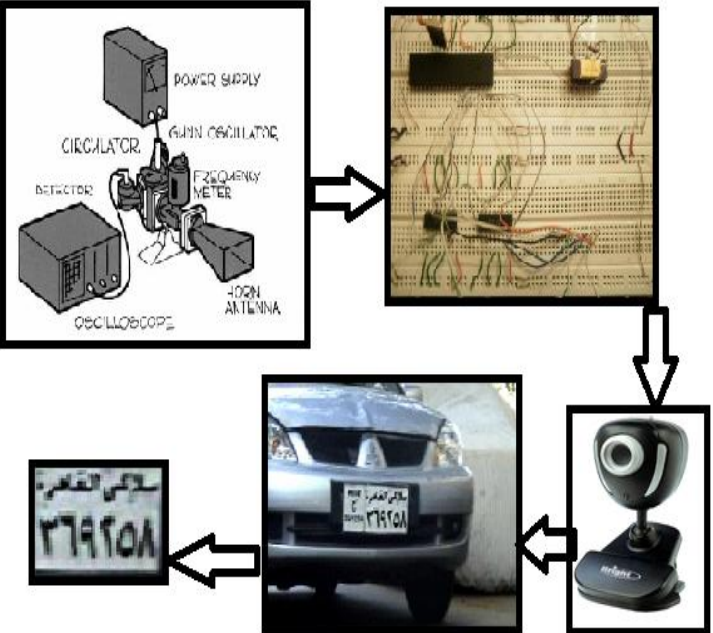
\includegraphics[width=0.45\textwidth]{figure1.png}
\end{figure}

\subsection{Project requirements:}
\begin{itemize}
	\item Information about Radar system.
	\item Radar wave generator circuit.
	\item Analogue to digital interface.
	\item Software for reading from the parallel port.
	\item Software for speed calibration.
	\item Software for image processing and determining the
	plate's contents.
\end{itemize}

\section{Methodology}
\noindent The main goal of this project is to minimize the number of
accidents per years, which occurs all over the roads, by
punishing the drivers that cross the speed limits. So we can
achieve this goal by following some steps to get this
idea.We use the radar to detect a moving car along the road
which the radar will be located. After that by the output of
the radar circuit, we get the output voltage and convert it to
digital form that will be used for measuring the car's speed.
Then the next phase is to order the camera by the input
value of the speed of the car to Taking a photo for the car if
it moving over speed. After saving the image of the car, we
make a number of operations that will be helpful for
analyzing the image, and detect the plate contents to report
it. The last part of the system is to take details of the car's
plate after extract the contents of the plate and sending the
car details to the responsible authority.

\section{Project objectives}
\subsection{HARDWARE \& NETWORK PLATFORMS:}
\noindent We will use for converting from analogue to digital a specific
hardware elements that will help and make it more simple for
implementing the hardware. We will use a microcontroller
for converting from analogue to digital.
\subsection{ Programming Languages:} 
\begin{itemize}
	\item We will use micro C for the program of the
	microcontroler which will be used for analogue
	to digital converter(ADC).
	\item Proteus for circuit simulation.
	\item Csharp and Matlab for inetrface.
	\item Matlab for calibration and license plate
	recognetion(LPR).
\end{itemize}
\subsection{KEY PROJECT BENEFITS:}
\begin{enumerate}
	\item Detect the speeding cars automatically.
	\item Using radar to measure speed of the car to
	avoid accident.
	\item Reduce human element which reduce errors.
	\item Easy handling and low cost.
	\item Make the road safer.
\end{enumerate}
\noindent Now we will speak about each one of the system
componentsto describe every operation in each part and how
it will be connected wih the other phase.
Chapter 2 will be about the radar circuit,its components and
the doppler shift which is the main idea of the radar operation
In chapter 3, chapter 4 we will mention in it how to design
the hardware interface and how it will operate to convert the
output analogue signal from the radar circuit to digital form
to can be easly recognized by the computer by attached the
parallel cable with the interface and the computer.
Chapter 5 will be about when the camera will picture the
moving cars, recognizing informationof the plate of the car
and send these information automaticaly by e-mail to
responsible authority.
At chapter 6 , software engineering is about the flow chart of
the system, constraints and the duration and tasks
implementation.






%
\chapter{LITERATURE REVIEW}
\label{chapter:Literature Review}

%: ----------------------- paths to graphics ------------------------


\ifpdf
    \graphicspath{{2_LiteratureReview/figures/PNG/}{2_LiteratureReview/figures/PDF/}{2_LiteratureReview/figures/}}
\else
    \graphicspath{{2_LiteratureReview/figures/EPS/}{2_LiteratureReview/figures/}}
\fi

% ----------------------------------------------------------------------
%: ----------------------- introduction content -----------------------
% ---------------------------------------------------------------
\section{Background}
There are various techniques of ..................
\section{AMB Control} 
AMB is inherently unstable nonlinear dynamical system. Thus, .........
\section{AMB Design}
Recently, an apparent clear trend in magnetic bearing and bearingless motors design could be noticed. Some researchers ...

This project work closes these gaps in the previous works by ........
\newpage

% ----------------------------------------------------------------------



	
\chapter{Radar}
\label{chapter:Radar}

%: ----------------------- paths to graphics ------------------------

\ifpdf
\graphicspath{{3_Radar/figures/PNG/}{3_Radar/figures/PDF/}{3_Radar/figures/}}
\else
\graphicspath{{3_Radar/figures/EPS/}{3_Radar/figures/}}
\fi

%: ----------------------- contents from here ------------------------
This chapter presents ...

\section{SD}

........

\section{SYD}
\noindent The proposed system is designed using the procedure given in ..............\\

\underline{STEP 1:} Arm and .......:

For payload and arm with the specifications given in Table \ref{Tabel_Armandpaylaod}, the maximum load Torque, $T_{Lmax}$, when the arm is horizontal, is calculated from the following equation:
\begin{equation}
	\label{eqloadtorque}
	T_{Lmax} = (0.15\ m_p + 0.075\ m_a)\ g
\end{equation}
Hence, the maximum load torque is equal 0.71 Nm.
\begin{table}[t]
	\caption{\textbf{Arm and payload parameters}}
	\centering
	\label{Tabel_Armandpaylaod}
	\begin{tabular}{|l|c|c|}
		\hline
		& \textbf{Payload} & \textbf{Arm} \\  \hline
		Dimension (mm) & 40x40x20  & 150x40x10 \\  \hline
		Mass (kg) & $m_p$ = 0.25  & $m_a$ = 0.47   \\   \hline
		C.G. Location (m) & 0.15 & 0.075	\\    \hline
	\end{tabular}
\end{table}
\\ 
\underline{STEP 2:} ...........:
.................... See Appendix \ref{appendA}.


\section{MS} 
\label{Measurement Sensors}
\noindent In this system...........
Nevertheless, ............

The second type ........... The most common sensor for this function is ............ shown in Fig. \ref{fig:gapsensor}.
\begin{figure}[!h!t]
	\centering
	\subfigure[]{
		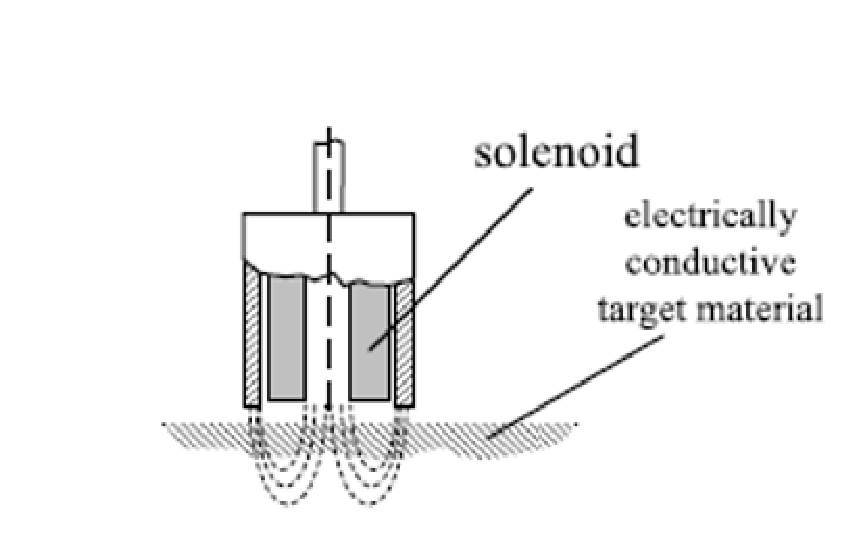
\includegraphics[width=5cm, height=4cm]{gap_sensor_1.eps}
	} 
	\subfigure[]{
		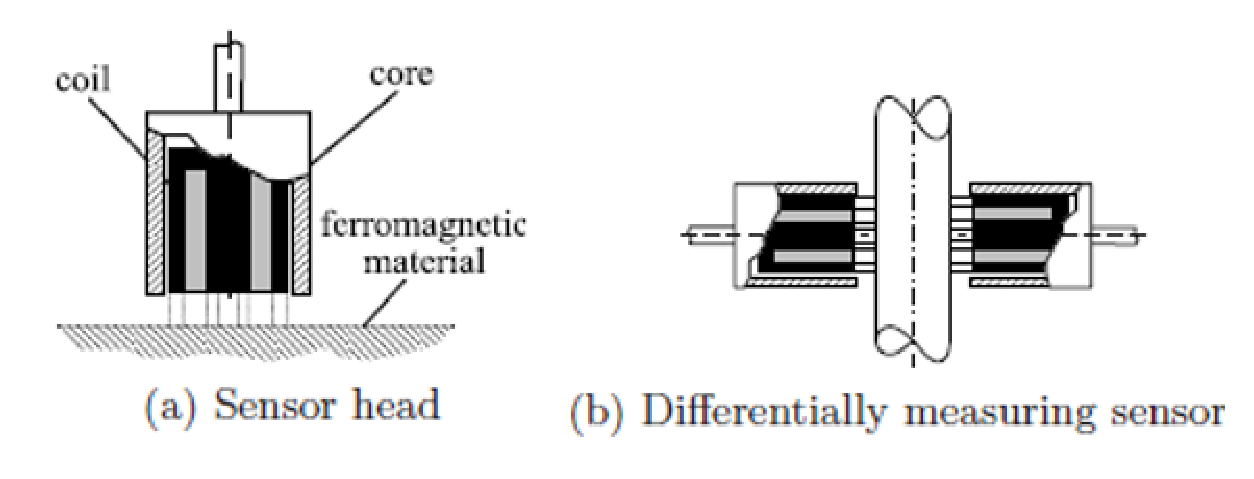
\includegraphics[width=8cm, height=4cm]{gap_sensor_2.eps}
	}
	\caption{Air gap measuring sensors (a) Eddy current displacement sensor, (b) Inductive displacement sensor.}
	\label{fig:gapsensor}
\end{figure}


\section{ABC} 
.......................
\subsection{SUB1-ABC}
.........................

\subsection{SUB2-ABC}
............................


% ---------------------------------------------------------------------------
%: ----------------------- end of thesis sub-document ------------------------
% ---------------------------------------------------------------------------
			
\chapter{SYSTEM DYNAMIC MODEL} 
\label{chapter:SystemMathematicalModeling}

%: ----------------------- paths to graphics ------------------------

\ifpdf
    \graphicspath{{4_SystemMathematicalModeling/figures/PNG/}{4_SystemMathematicalModeling/figures/PDF/}{4_SystemMathematicalModeling/figures/}}
\else
    \graphicspath{{4_SystemMathematicalModeling/figures/EPS/}{4_SystemMathematicalModeling/figures/}}
\fi

%: ----------------------- contents from here ------------------------

This chapter presents ...........
\section{B}
\noindent The .............:

\begin{equation}
\label{eq1BLDC}
\begin{split}
\left[\begin{array}{c} v_a \\ v_b \\ v_c \end{array}\right] & = \begin{bmatrix}
R & 0 & 0 \\
0 & R & 0 \\
0 & 0 & R
\end{bmatrix}  \left[ \begin{array}{c} i_a \\ i_b \\ i_c \end{array} \right]\\
& +\begin{bmatrix}
L_s-L_m & 0 & 0 \\
0 & L_s-L_m & 0 \\
0 & 0 & L_s-L_m
\end{bmatrix} \frac{d}{dt} \left[ \begin{array}{c} i_a \\ i_b \\ i_c \end{array} \right] + \left[ \begin{array}{c} e_a \\ e_b \\ e_c \end{array} \right] 
\end{split}
\end{equation}

....................with a maximum magnitude of $\pm$ 1. 

\section{AMBM}
\subsection{ Model.} 
\label{AMB Nonlinear Model}
..............................

%++++++++++++++++++++++++++++++++++++++++++++++++++++++++++++++
\section{MPA}
\label{Micro-Positioning}
...................
\begin{equation}
\label{m1}
^1H_2 =  \begin{bmatrix}
\begin{array}{ccc|c}
1 & 0 & 0 &  ^1x_2 \\
0 & 1 & 0 &  ^1y_2 \\
0 & 0 & 1 &  ^1z_2 \\
\hline
0 & 0 & 0 &  1 \\
\end{array} 
\end{bmatrix}
\end{equation}

where, $^1x_2$, $^1y_2$ and $^1z_2$ are constants lengths.

%: ----------------------- end of thesis sub-document ------------------------
% ---------------------------------------------------------------------------



\chapter{CONTROLLER DESIGN} 
\label{chapter:ControllerDesign}
\label{controller design}
%: ----------------------- paths to graphics ------------------------

\ifpdf
    \graphicspath{{5_ControllerDesign/figures/PNG/}{5_ControllerDesign/figures/PDF/}{5_ControllerDesign/figures/}}
\else
    \graphicspath{{5_ControllerDesign/figures/EPS/}{5_ControllerDesign/figures/}}
\fi


%: ----------------------- contents from here ------------------------
This Chapter................
\section{Angle}
\noindent A ................

\begin{equation}
\label{fblin2}
U_{\phi} = \ddot{\phi}_d + K_p\ e + K_d\ \dot{e} + K_i\ \int\limits_{0}^{t}e\ dt
\end{equation}
.............................
\section{Control}
with respect to the cost function
\begin{equation}
\label{lqr2}
J = \int\limits_{0}^{\infty} \left[ \begin{array}{c} x(t) \\ u(t) \end{array}  \right]^T \begin{bmatrix}
q & s   \\
s^T & r \\
\end{bmatrix}\left[ \begin{array}{c} x(t) \\ u(t) \end{array}  \right]
\end{equation}


% ---------------------------------------------------------------------------
%: ----------------------- end of thesis sub-document ------------------------
% ---------------------------------------------------------------------------

	

\chapter{Results and Discussion} 
\label{chapter:simu}

%: ----------------------- paths to graphics ------------------------


\ifpdf
    \graphicspath{{6_Resultsanddiscussion/figures/PNG/}{6_Resultsanddiscussion/figures/PDF/}{6_Resultsanddiscussion/figures/}}
\else
    \graphicspath{{6_Resultsanddiscussion/figures/EPS/}{6_Resultsanddiscussion/figures/}}
\fi


%: ----------------------- contents from here ------------------------

This chapter ............................

%----------
%: -------- end of thesis sub-document -----------


\chapter{CONCLUSIONS} 
\label{chapter:Conclusions}


% ----------------------- paths to graphics ------------------------


\ifpdf
    \graphicspath{{7_Conclusions/figures/PNG/}{7_Conclusions/figures/PDF/}{7_Conclusions/figures/}}
\else
    \graphicspath{{7_Conclusions/figures/EPS/}{7_Conclusions/figures/}}
\fi


% ----------------------- contents from here ------------------------
\section{Conclusions}
\noindent Now, we are capable of detecting the moving cars and capture the
over speeding cars to recognize the license plate of the car to send
it to the related authority. Another feature has been added to the
system, is to extract the Arabic numbers to send the license plate
contents to the related authority by sending an e-mail with an
attached text file which contains the Arabic numbers. This feature
will reduce the size of the attached file which will be sent to make
it easier and faster to be received by the related authority.

\section{ Future work:}
 \subsection{Professional cameras:}
\begin{enumerate}
	\item \textbf{Professional cameras for face detection:}\\
	Nowadays people are aware of the need of vehicle
	security due to the fact that they are various cases of car
	robbery. Therefore it is incumbent upon us to increase
	the level of securities. To make the system more secure,
	the system is recommended to integrate with face
	detection. This is means instead of identifying driver
	with their plate, it also important to identify by her or
	his face.\\
     We can do this by using a professional camera that
	contain a face detect applications, nowadays there are
	growing number of digital cameras now include a Face
	Recognition mode. The camera detects faces in a scene
	and then automatically focuses (AF) and optimizes
	exposure (AE).
	\item \textbf{- Professional camera to upgrade the image quality:}
	We want to use more professional cameras to improve
	the image quality to be easier to recognize the plate
	numbers.
	\begin{figure}[h]
		\centering
		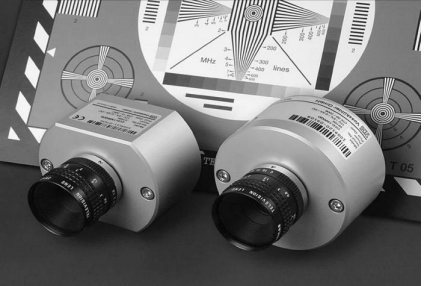
\includegraphics[width=0.45\textwidth]{figure2.png}
		\caption*{Color-ccd-digital camera	}
	\end{figure}
	\item \textbf{- Hard and waterproof cameras:}\\
	We can use hard cameras to avoid damages because
	they are located in the streets so they can be damaged
	by any one, but if we use hard material or it can be put
	in hard box it will be safer to avoid damage. Also, we
	want to use waterproof cameras because it is located in
	the open air, so maybe it will be rained.
	\item \textbf{Location of the camera:}\\
	The camera to vehicle distance around 40 feet. This
	system is able to detect license plate area for all the
	vehicles. We want to put the camera in the middle of
	the road to be able to detect any vehicles.
\end{enumerate}

\subsection{ Identification of segmented character:}
Save the segmented characters and numbers in one text file which
may be by comparing the segmented image with an already saved
one or compare it to a matrix of images in order to be ready for
database.
\begin{enumerate}
	\item \textbf{-Recognition System of Arabic Characters}\\
	At this stage, a recognition system of Arabic characters
	is presented, using a structural method based on the
	extraction of primitives (holes, concavities, characters
	form, existence of points, position of point, and number
	of connected components). This stage is performed in
	two steps;
	Characters classification and identification.\\
	\uline{\textbf{a$)$ Characters classification:}}\\
	The character classification takes as criteria the
	concavities in different directions, and the holes, which
	represent the main characteristics (morphological ones).
	The choice of these characteristics enables the system
	to work with multi-sized characters without having to
	perform an eventual normalization.
\end{enumerate}
\noindent The inner details of characters such as the presence of holes and
concavities are obtained to produce some unique features for some
Arabic characters. The holes feature is used to identify some
characters or resolve any ambiguity in the recognition phase. The
presence or absence of the hole, concavities direction, and dots are
powerful features for enhancing the implemented Arabic
recognition system. 

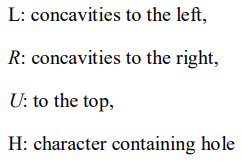
\includegraphics{ff.png}\\
We can compute each character's class using this formula:
\begin{equation*}
	class=2^0H+2^1U+2^2R+2^3L
\end{equation*}

\begin{figure}[h]
	\centering
    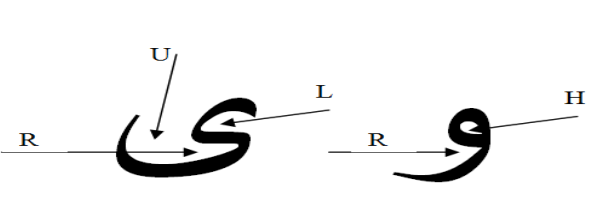
\includegraphics[width=0.5\textwidth]{aa.png}
\end{figure}

We must study the intensity of top and down parts, if the character
has the intensity of top part is smaller or greater than the intensity
of the down part. 
\begin{figure}[h]
	\centering
	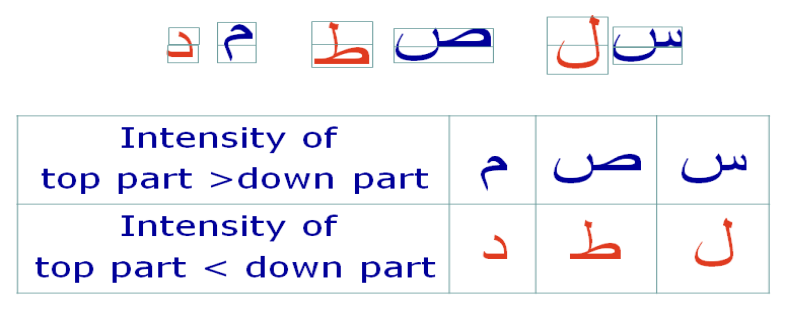
\includegraphics[width=0.6\textwidth]{bb.png}
\end{figure}
\\
\uline{\textbf{b$)$Characters identification:}}\\
-Egyptian new license plates use only 17 characters
from 28.
\begin{figure}[h]
	\centering
	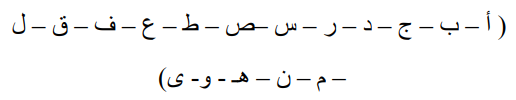
\includegraphics[width=0.5\textwidth]{ee.png}
	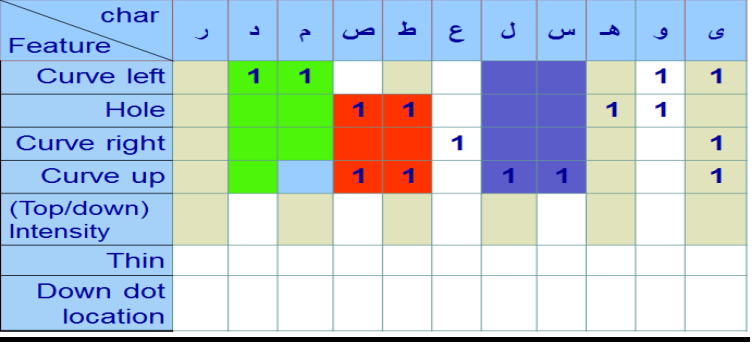
\includegraphics[width=0.7\textwidth]{cc.png}
	\caption*{After that we can identify any Arabic plate character.}
\end{figure}
\subsection{Creating a database of the system:}
We use to create a data base for all the cars plate numbers and their
owner identity .We use SQL to create a database for the car plate
number and the name of the owner and his penalty.
\begin{figure}[!h]
	\centering
	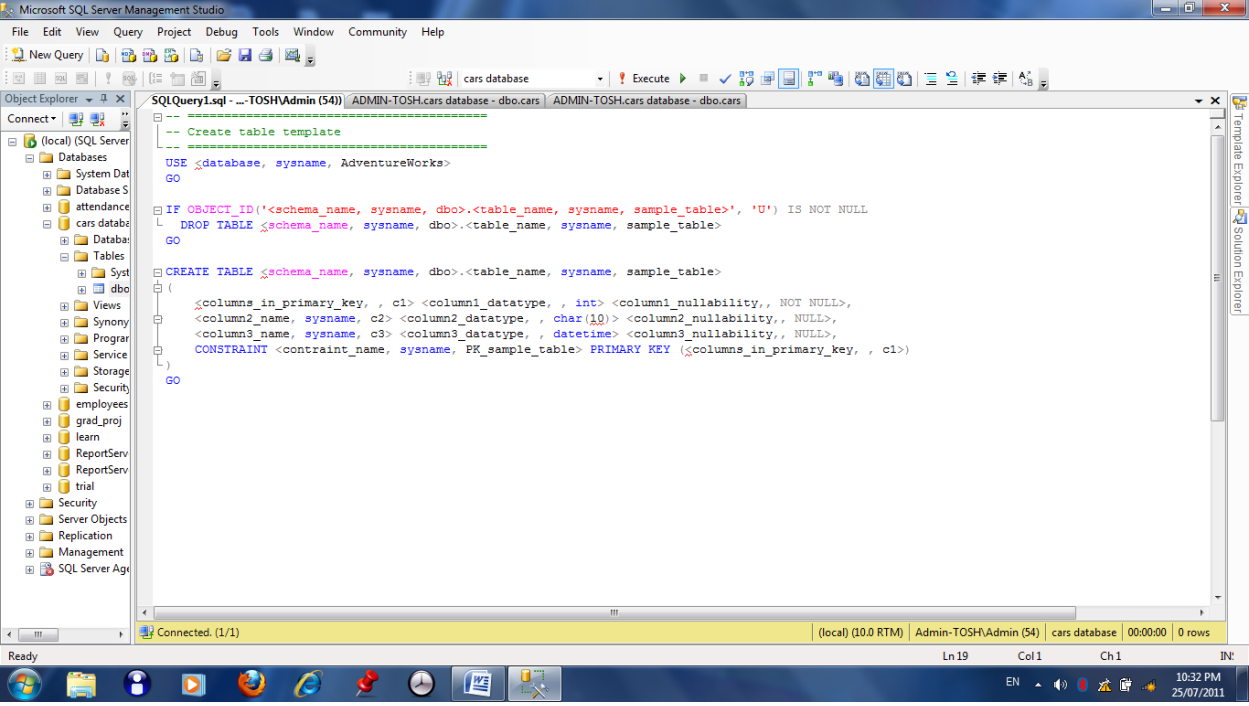
\includegraphics[width=0.64\textwidth]{dd.png}
\end{figure}
\subsection{Sending SMS}
\noindent After building the database system and detecting the license plate
numbers, we will use these numbers to compare it with the data
base elements to extract the car owner's telephone number. After
that we will use a software program to send an automatic SMS to
the car owner to inform him that he has been crossed the limit
speed. This program will be designed by C\# and the main function
of the operation will be:\\
\textcolor{red}{sms = "You've received a speeding ticket!$\backslash$nSpeed: " + 150 +
	"$\backslash$nPlace: Alexandrai ST @ 100 KM$\backslash$nTime: " + DateTime.Now + "$\backslash$nBill: "
	+ 500 + " LE";\\
	sendSMS("COM19", "0105471662", sms);} \\
We have first to attach the mobile phone to the COM port, and
defining it by task manager. Then the SMS will be sent to the
required number via the attached mobile phone.
\subsection{Moving and non moving cars}
\noindent Use the LPR (license Plate Recognition) in monitoring roads and
detect moving parts by using video segmentation this system is
used in south Africa where we can catch stolen cars by
automatically recognize the car plate and search it in a database, if
the passing car is identical with one of those in the black list it
sends the location to the authorized persons. Detection of moving
vehicles simplifies the processing on subsequent analysis steps.
Due to dynamic changes in natural scenes such as sudden
illumination and weather changes, repetitive motions that cause
clutter (tree leaves moving in blowing wind), motion detection is a
difficult problem to process reliably. Frequently used techniques
for moving vehicle detection are background subtraction, statistical
methods, temporal differencing and optical flow. In case we used
the Background subtraction which is particularly a commonly used
technique for motion segmentation in static scenes, it attempts to
detect moving regions by subtracting the current image pixel-bypixel from a reference background image that is created by
averaging images over time in an initialization period, The pixels
where the difference is above a threshold are classified as
foreground. After creating a foreground pixel map, some
morphological post processing operations such as erosion, dilation
and closing are performed to reduce the effects of noise and
enhance the detected regions. The reference background is updated
with new images over time to adapt to dynamic scene changes.
While in case we used Statistical Methods which is more advanced
methods that make use of the statistical characteristics of
individual pixels have been developed to overcome the
shortcomings of basic background subtraction methods. These
statistical methods are mainly inspired by the background
subtraction methods in terms of keeping and dynamically updating
statistics of the pixels that belong to the background image
process. Foreground pixels are identified by comparing each
pixel's statistics with that of the background model. This approach
is becoming more popular due to its reliability in scenes that
contain noise, illumination changes and shadow Finally both
methods can detect the moving vehicle we can use one of them to
reach our target and distinguish between the moving cars and the
non-moving ones for any following purposes.


% ---------------------------------------------------------------------------
% ----------------------- end of thesis sub-document ------------------------
% --------------------------------------------------------------------------- 


%: ------------- bibliography ---------------

\renewcommand{\bibname}{REFERENCES}
\bibliography{10_backmatter/references} 
\bibliographystyle{Latex/Classes/IEEEtran}

%-------------appendix----------------------
\renewcommand{\chaptermark}[1]{%
	\markboth{\MakeUppercase{\appendixname\ \thechapter}}%
	{\MakeUppercase{#1}}
}

\fancyhead[RE,LO]{}
\appendix

\chapter{Brushless DC Motor} 
\label{appendA}

\ifpdf
    \graphicspath{{8_Appendices/figures/PNG/}{8_Appendices/figures/PDF/}{8_Appendices/figures/}}
\else
    \graphicspath{{8_Appendices/figures/EPS/}{8_Appendices/figures/}}
\fi

% ----------------------- contents from here ------------------------

\begin{figure}
	\begin{center}
		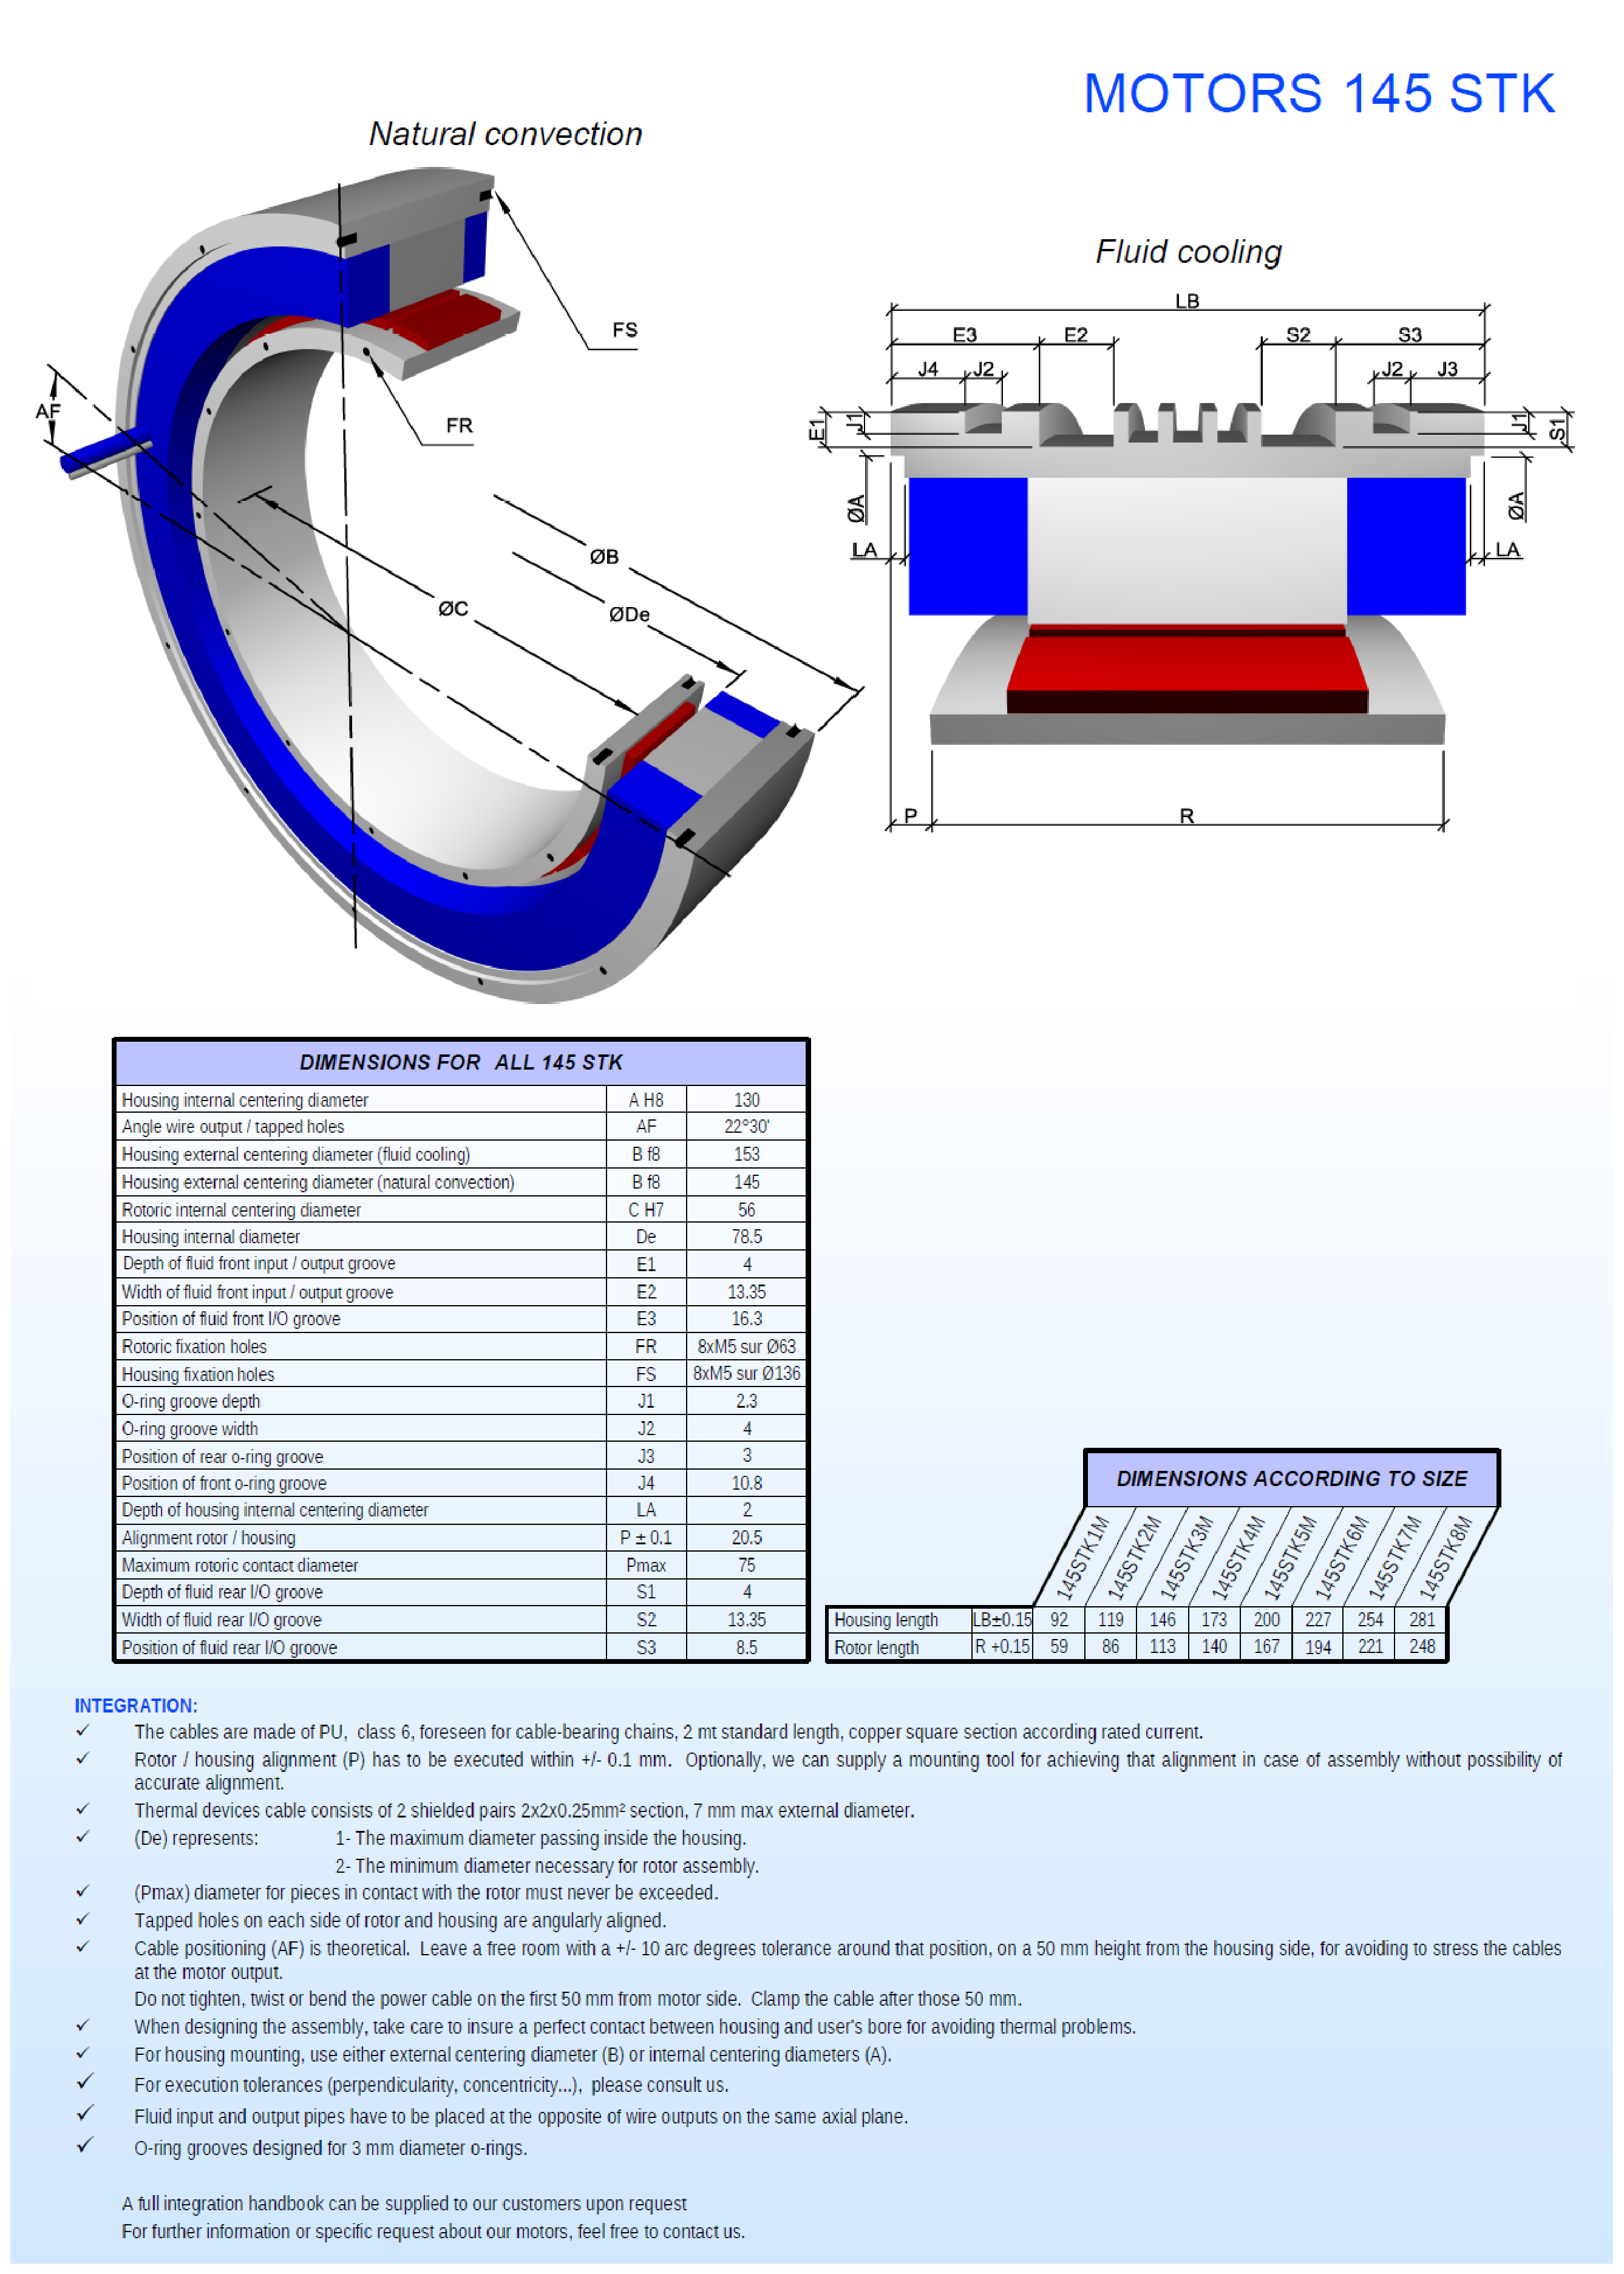
\includegraphics[width=15cm]{BLDC_page_1.eps}
		\caption{BLDC motor data sheet page 1 of 3.}
		\label{fig:BLDC1}
	\end{center}
\end{figure}



\end{spacing}

\cleardoublepage
\newpage\null\thispagestyle{empty}\newpage

\end{document}